W poniższym rozdziale zawarty został opis teoretyczny dziedziny eye-trackingu, jak również analiza algorytmów wykrywania fiksacji wykorzystanych do przeprowadzenia badań.
\section{Eye-tracking}
W następującej sekcji zaprezentowana zostanie technologia eye-trackingu, oraz jej zastosowania.\\[\baselineskip]
Jak wspomniano we wstępie do pracy, rozwój okulografii w przeciągu ostatnich kilkudziesięciu lat pozwala nam przeanalizować sposób w jakim operują ludzkie procesy obserwacji oraz sposobu rozpoznawania obrazu. Analiza tych procesów umożliwia badającym na wykorzystywanie wyników badań w zastosowaniach komercyjnych, np. badanie sposobu patrzenia na jezdnię w trakcie jazdy pojazdem \cite{CarSteering}, analiza psychologiczna \cite{GazeEyeTrackingSolutions} czy też w reklamach \cite{Advertising}.\\[\baselineskip]
W celu przetworzenia danych z urządzenia do dalszej analizy stosuje się typowo dwie wartości: fiksacje, czyli miejsca, na których badana próbka wzroku się skupiła, oraz sakady, szybkie ruchy pomiędzy fiksacjami. Podział ten został odkryty w XIX wieku we Francji za pomocą obserwacji fizycznych, ponieważ zauważono, że ludzkie oko podczas czytania nie porusza się płynnie, a wykonuje "skoki" pomiędzy obszarami tekstu. Przykład takiego ruchu oraz punktów skupienia można zaobserwować na rysunku \ref{fig:fiksacje}.
\begin{figure}[H]
    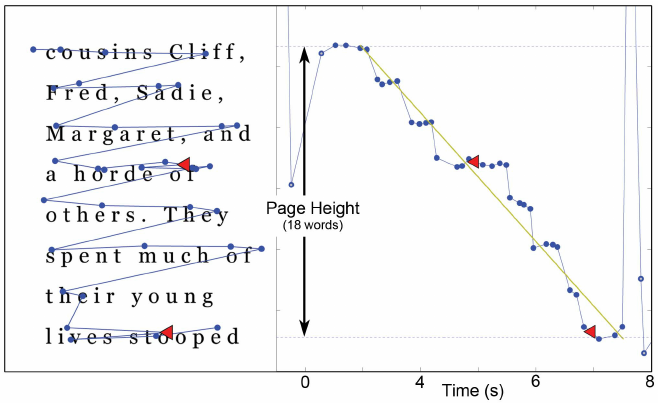
\includegraphics[width=\linewidth]{resources/fixation_example.jpg}
    \caption{Przykład fiskacji i sakad na tekście}
    \label{fig:fiksacje}
\end{figure}
Analiza fiksacji między innymi poprzez translacje danych ruchu oka z urządzenia wejściowego na fiksacje, co pozwala również określić sakady na pomiarze. Daje to możliwość pozbycia się zbędnych danych z próbki, takich jak sakad, oraz pomniejszych ruchów oka, które mogły nastąpić przy niedokładnym pomiarze, czy mikroskopijnym ruchu oka. Zezwala to nam na zmniejszenie rozmiaru danych, poprzez zbijająnia rzeczywistych fiksacji do jednego, większego punktu danych. Najczęściej otrzymane wartości są wykorzystywane do metryk pomiaru typu czas fiksacji, prędkości i amplitudy sakad, jak również miary pomiędzy fiksacjami a sakadami. Jednak cytując \cite{Main} \emph{"w większości badań naukowych, dane z sakad nie stanowią aż takiej przydatności"}.\\[\baselineskip]
Wyniki algorytmów wykrywania fiksacji są wynikami typowo statystycznymi, tzn. możemy określić ile wystąpiło fiksacji, a przez to ile elementów jest sakadami, ale dalsza analiza danych należy do badającego. Stwarza to problem interpretacji danych, zgodnie z \cite{Main} \emph{"jednym ze sposobów walidacji tych algorytmów jest porównanie wynikowych fiksacji z wrażeniami wizualnymi obserwującego"}.
\subsection{Typy algorytmów wykrywania fiksacji}
Wyróżniamy trzy główne rodzaje algorytmów wykrywania fiksacji: prędkościowe, dyspersyjne oraz powierzchniowe. Algorytmem prędkościowym możemy nazwać algorytm, który analizuje punkty pod kątem różnicy prędkości pomiędzy nimi, biorąc pod uwagę, iż fiksacje posiadają niską prędkość pomiędzy swoimi punktami, a sakady wysoką. Algorytmy dyspersyjne bazują na odległościach rozproszenia między punktami, gdzie fiksacje posiadają je małe, a sakady duże. Algorytmy powierzchniowe to algorytmy, których zadaniem jest identyfikacja punktów w wybranych powierzchniach zainteresowania (z ang. \textit{Area of Interest - AOI}). \emph{do dopisania}
\section{Wybrane algorytmy}
Celem poniższego podrozdziału jest opis teoretyczny algorytmów wykrywania fiksacji zastosowanych w pracy. Opis teoretyczny wybranych algorytmów bazuje na pracy \cite{Main}.
\subsection{Algorytm I-VT}
Algorytm I-VT (z ang. \emph{Identification-Velocity Threshold}) jest przykładem algorytmu z grupy prędkościowych, jak wspomniano w poprzednim podrozdziale. Ze względu na małą złożoność algorytmu, jest on najprostszą metodą do zaimplementowania.\\

Pseudokod algorytmu I-VT zaprezentowano w tabeli \ref{tab:ivt}.
\begin{table}[H]
    \begin{tttabular}{|p{15cm}|}
        \hline
        Oblicz prędkości pomiędzy punktami dla każdego punktu w protokole.\\
        \smallskip
        Określ punkty poniżej progu jako fiksacje, a powyżej jako sakady.\\
        \smallskip
        Połącz wszystkie punkty fiksacji w grupy fiksacji, usuń wszystkie sakady.\\
        \smallskip
        Zmapuj każdą grupę fiksacji do punktu znajdującego się w środku każdej grupy.\\
        \smallskip
        Zwróć fiksacje.\\
        \hline
    \end{tttabular}
    \caption{Pseudokod algorytmu I-VT}
    \label{tab:ivt}
\end{table}
\subsection{Algorytm I-DT}
\subsection{Uczenie maszynowe}
\section{Inne metody analizy okulograficznej}